
\documentclass[sigplan,screen]{acmart}


\input{cloudmask-report-format}

\begin{document}

\newcommand{\TITLE}{An Overview of MLCommons CloudMask: \\ Related Research and Data \\ {\normalsize Version 1.0}}

\title[Overview of MLCommons CloudMask: Related Research]{\TITLE}

\author{Gregor von Laszewski}
\email{laszewski@gmail.com}
\orcid{0000-0001-9558-179X}
\authornote{MLCommons authorized submitting author}
\affiliation{%
  \institution{University of Virginia}
  \streetaddress{Biocomplexity Institute and Initiative\\
Town Center Four\\
994 Research Park Boulevard}
  \city{Charlottesville}
  \state{VA}
  \postcode{22911}
  \country{USA}
}

\author{Ruochen Gu}
\email{bill.ruochen.gu@gmail.com}
\affiliation{%
  \institution{}
  \streetaddress{}
  \city{Shanghai}
  \state{}
  \postcode{}
  \country{CN}
}

\renewcommand{\shortauthors}{von Laszewski et al.}

\begin{abstract}

In this paper, we summarize some of the ongoing research activities in cloud masking as well as in the MLCommons Science Working Group.
Cloud masking is a crucial task that is well-motivated for meteorology and its applications in environmental sciences. Given satellite images, cloud masks are generated such that each pixel is labeled to either have cloud or clear sky. 

\end{abstract}



\begin{comment}
\begin{CCSXML}

\end{CCSXML}

\ccsdesc[500]{Computer systems organization~Embedded systems}
\ccsdesc[300]{Computer systems organization~Redundancy}
\ccsdesc{Computer systems organization~Robotics}
\ccsdesc[100]{Networks~Network reliability}

\end{comment}

%%
%% Keywords. The author(s) should pick words that accurately describe
%% the work being presented. Separate the keywords with commas.
\keywords{cloudmask, cloudmesh, datasets}


\received[Version from]{8. June , revised 14 November, 2023}

\begin{comment}
    
\begin{center}
{\huge\bf \TITLE}
\end{center}

% \listoftodos

\tableofcontents
\listoffigures
\listoftables

\clearpage
\end{comment}

\maketitle


%%%%%%%%%%%%%%%%%%%%%%%%%%%%%%%%%%%%%%%%%%%%%%%%%%%%%
\section{MLCommons Cloud Mask Activities}
%%%%%%%%%%%%%%%%%%%%%%%%%%%%%%%%%%%%%%%%%%%%%%%%%%%%%

This activity is conducted as part of the work with MLCommons \cite{Farrell2021MLPerfHA}. 
It is part of the research conducted by MLCommons Science Working Group \cite{www-mlcommons-science-github}. 
We hope that others will contribute to this 
document to enhance its scope. Please contact Gregor von Laszewski (laszewski@gmail.com) 
so we can coordinate with you.

At this time we are aware of a number activities using MLCommons cloudmask benchmark.


\begin{enumerate}
\item The original benchmark has been contributed by Rutherford Labs Samual Jackson  and Juri Papaya \cite{Thiyagalingam2022AIBF}.
The reference implementation is based on U-Net \cite{Ronneberger2015UNetCN} mode. 

\item An activity from Junji Yin to benchmark the Cloudmask MLCommons benchmark on PEARL \cite{Thiyagalingam2022AIBF}.

\item The activity by Gregor von Laszewski on UVA Rivanna. This activity contains significant contributions. 

    \begin{enumerate} 

    \item the introduction of target directories that showcase how to use templates to run cloudmask on various HPC machines, but also dgx station and a Linux desktop with an NVIDIA card.

    \item the modification of the code to include enhanced timers throughout the code to measure the different parts.

    \item The use of the Cloudmesh StopWatch to provide easy human readable timers that can also be parsed with little effort through an export as CSV data.

    \item The development and use of a hyper-parameter permutation framework that allows the code to be run easily with different parameters from epochs, batch sizes, learningrate, and more. This work is also reused in other MLCommons Science benchmarks \cite{las22-cloudmesh-cc-reu}.

    \item The development of a workflow system that allows the use of hybrid compute resources through templates \cite{las-2023-escience-cloudmask} .

    \item The application of these efforts in eductaion as documented for another application in \cite{las-2023-mlcommons-edu-eq}.

    \item the hosting of a development repository for the MLCommons cloudmask code as part of the MLCommons Science Working Group \cite{github-laszewsk-mlcommons}.

    \item The execution of many performance experiments.

\end{enumerate}

\item The activity by a team at NYU while modifying the code with early stoppage which is currently in draft and builds on the activities from the UVA and Rutherford Lab. This includes a modification of the original code while using the accuracy value introduced by S. Jackson, J. Papaya, and G. v. Laszewski.

The submission of benchmarks is coordinated through a bash script that is replication a small number of features from the previous more comprehensive activity. This work, was focused on the introduction of early stoppage into the model training. The experiment contains a more limited number of experiments in contrast to the previous effort. A report is under preparation. Several versions of the report were started such as \cite{las23-cloudmask}. The latest report si not yet available.

\end{enumerate}


%%%%%%%%%%%%%%%%%%%%%%%%%%%%%%%%%%%%%%%%%%%%%%%%%%%%%
\section{Overview of Related Work}
%%%%%%%%%%%%%%%%%%%%%%%%%%%%%%%%%%%%%%%%%%%%%%%%%%%%%

Several methods have been used for cloudmask ranging from rule-based \cite{Saunders1986AnAS,Saunders1988AnIM,Merchant2005ProbabilisticPB, Zhu2012ObjectbasedCA} to deep learning \cite{Li2019DeepLB,Domnich2021KappaMaskAC,Yan2018CloudAC,WIELAND2019111203,JEPPESEN2019247}. Some of the rule based techniques have been thresholding \cite{Saunders1986AnAS,Saunders1988AnIM} and Bayesian masking \cite{Merchant2005ProbabilisticPB}. Bayesian masks use the Bayes' theorem and prior meteorology information to provide probabilities for each pixel having a cloud or not. Using these probabilities and applying them to a given image, a cloud mask can be generated. On the other hand, deep learning methods\cite{Li2019DeepLB,Domnich2021KappaMaskAC,Yan2018CloudAC,WIELAND2019111203,JEPPESEN2019247} use computer vision models and treat the task as that of image segmentation to generate these cloud masks. The most widely used model is the U-Net \cite{Ronneberger2015UNetCN} model which is pre-trained and designed for such a task, especially for large images.


%%%%%%%%%%%%%%%%%%%%%%%%%%%%%%%%%%%%%%%%%%%%%%%%%%%%%
\section{Related Work}
%%%%%%%%%%%%%%%%%%%%%%%%%%%%%%%%%%%%%%%%%%%%%%%%%%%%%

To produce these cloud masks, the traditional approaches have been: thresholding \cite{Saunders1986AnAS,Saunders1988AnIM} and Bayesian\cite{Merchant2005ProbabilisticPB} methods. Thresholding methods consist of several threshold tests where spectral and spatial properties of the images are compared with ranges that are believed to be indicative of a {\em clear-sky} pixel. And those other pixels that are not labeled as {\em clear-sky} are flagged as {\em cloudy} pixel. This method was widely used from the late 1980s to the early 2000s \cite{Merchant2005ProbabilisticPB}. The gradual transition away from threshold tests was due to its long-criticized limitations: firstly, threshold settings rely on domain expertise about indicators of cloudiness that may not be objective, which also makes later modification and updates difficult; secondly, thresholds provide users no flexibility in the trade-off between SST coverage and SST bias; third, threshold tests do not make use of all available prior information. These shortcomings of thresholding methods are improved by later developed Bayesian methods \cite{Merchant2005ProbabilisticPB}.


Bayesian methods deduce the probability of a clear sky over each pixel by applying Bayes' theorem. As a result, these Bayesian approaches are fully probabilistic and deduce pixels based on prior information and observations in images. Compared to threshold tests, Bayesian methods achieve a better accuracy in predicting pixels' cloudiness, offering generality and conceptual clarity in its approach, and enhancing maintainability and adaptability largely \cite{Merchant2005ProbabilisticPB}. 

More recently, the rise of deep learning has led to the use of CNNs for generating these cloud masks. CNNs have achieved superior performance due to their ability of automatic feature extraction. \cite{WIELAND2019111203} have shown the use U-Net to generate cloud masks and have achieved higher results compared to the state-of-the-art rule-based approach Fmask  \cite{Zhu2012ObjectbasedCA}. \cite{JEPPESEN2019247} introduced Remote Sensing Network (RS-Net), an architecture based on U-Net for cloud masking, and also have shown to achieve higher performance compared to Fmask \cite{Zhu2012ObjectbasedCA}.

KappaMask \cite{Domnich2021KappaMaskAC} was another U-Net based CNN model that outperformed the rule-based Fmask algorithm. MSCFF \cite{Li2019DeepLB} is a CNN model that uses an encoder-decoder model to extract high-level features. MCSFF also outperforms Fmask on several satellite datasets. All these models have reported their performances on several satellite images such as Sentinel-2, Landsat, etc., and also make use of human-annotated (some assisted by software) ground truth values. On the contrary, the cloud-masking benchmark makes use of Sentinel-3's images and uses Bayesian masks as the ground truth. To our best knowledge, there is no previous work done using Sentinel-3 images except the reference implementation provided by MLCommons Science Working Group that achieves 92\% classification accuracy on the test set.

We provide a short overview of related work in regard to the observation data gathering. The data is gathered with different instruments/satellites  The list of datasets is shown in Table \ref{tab:datasets}. 

\begin{table*}[htb]
    \centering
    \caption{This table presents the several methods used for cloud masking with their respective dataset, ground truth, and performance.}
    \label{tab:datasets}
    \resizebox{1.8\columnwidth}{!}{
    \begin{tabular}{|l|c|l|l|l|l|}
    \hline
        {\bf} & {\bf Reference} & {\bf Dataset} & {\bf Ground-truth} & {\bf Model}  & {\bf Accuracy} \\ \hline
        1 & \cite{Merchant2005ProbabilisticPB} & ATSR-2 & Human annotation & Bayesian screening & 0.917\\ \hline
        2 & \cite{WIELAND2019111203} & Sentinel-2 & Software-assisted human annotation (QGIS) & U-Net & 0.90 \\ \hline
        3 & \cite{WIELAND2019111203} & Landsat TM & Software-assisted human annotation (QGIS) & U-Net & 0.89 \\ \hline
        4 & \cite{WIELAND2019111203} & Landsat ETM+ & Software-assisted human annotation (QGIS) & U-Net & 0.89 \\ \hline
        5 & \cite{WIELAND2019111203} & Landsat OLI & Software-assisted human annotation (QGIS) & U-Net & 0.91 \\ \hline
        6 & \cite{8401847} & GaoFen-1 & Human annotation & MFFSNet & 0.98, mIOU = 0.87 \\ \hline
        7 & \cite{Domnich2021KappaMaskAC} & Sentinel 2 & Software-assisted human annotation (CVAT) & KappaMask & 0.91 \\ \hline
        8 & \cite{JEPPESEN2019247} & Landsat 8 Biome and SPARCS & Human annotation & RS-Net & 0.956 \\ \hline
    \end{tabular}}

\end{table*}



%%%%%%%%%%%%%%%%%%%%%%%%%%%%%%%%%%%%%%%%%%%%%%%%%%%%%
\section{Dataset} 
%%%%%%%%%%%%%%%%%%%%%%%%%%%%%%%%%%%%%%%%%%%%%%%%%%%%%


The MLCommons benchmark used 180GB of satellite images from Sentinel-3 satellite images. The dataset consists of a total of 1070 images, both captured at day and night. The dataset comes with the train-test split where 90\% is used for training, and 10\% is used for testing. 
The images are of the dimension 1200 x 1500 with fifteen different channels. Three channels are used to represent brightness, six channels are used to represent reflectance, and six channels are used to represent radiance. However, for the benchmark, as provided in the reference implementation, only a total of nine channels, i.e., six channels of reflectance and three channels of brightness are used. 

\begin{figure*}[htb]

\centering\includegraphics[width=0.75\textwidth]{images/cloudmask-preprocessing-training-data.pdf}
\caption{The preprocessing of the training data.}
\label{fig:preprocessing-training}

\bigskip

\centering\includegraphics[width=0.75\textwidth]{images/cloudmask-preprocessing-testing-data.pdf}
\caption{The preprocessing of testing data}
\label{fig:preprocessing-testing}

\end{figure*}


\subsection{Preprocessing and postprocessing} According to the reference implementation, while training the U-Net model, the input images and their ground truths are first cropped and then divided into smaller sized $256 \times 256$ patches, keeping all the nine channels intact. After creating these patches of individual images, we get a total of $19,400$ images for training. Hereafter, we refer to patches as images. These images are further split into training and validation set using the $80/20$ split ratio, and then sent for training after shuffling. 
For the test set, the images are neither cropped nor shuffled. Overlapping smaller images(patches) of $256 \times 256$ are created both for the input image but not for the ground truth, and we get a total of $6300$ images. After getting the predictions from the model, these  $256 \times 256$ images are reconstructed to the original size and then evaluated with the ground truth. This entire preprocessing for training and inference are shown in Figure \ref{fig:preprocessing-training} and Figure \ref{fig:preprocessing-testing}.

\subsection{Training}

During training, the model takes an image of size $256 \times 256$, and generates a cloud mask of the same size. Once the cloud masks have been generated by the model during training, the accuracy is reported as the number of pixels that are correctly classified as cloud or not. 

\subsection{Inference}

During inference, the model first generates a cloud mask for each $256 \times 256$ image of testing data, where the input image goes through the same preprocessing step as described above for training. For each pixel in the image, the model outputs a probability of that pixel having clear-sky. Pixels that have a probability larger than 0.5 are labeled as clear-sky and the others cloudy. Then, those images are then reconstructed back to full size masks of dimension 1200*1500. 

The locations of the images used in the cloudmask inference are depicted in Figure~\ref{fig:frames-inference} as well as the centers in Figures~\ref{fig:frames-dot}.
Furthermore we display in Figure \ref{fig:frames-raw} the satellite images from the Sentinel-3 data base that reflect the locations where the inference images are located. Figure \ref{fig:frames-mask} shows the masks that we regenerated in the inference at the particular locations.
The Table \ref{tab:mask-table} shows the individual attributes for the specific locations identified by a counter.

\begin{figure*}[htb]
\centering\includegraphics[width=0.75\paperwidth]{images/inference-frames.pdf}
\caption{The location of the satellite images represented as frames used for inference.}
\label{fig:frames-inference}

\centering\includegraphics[width=0.8\paperwidth]{images/inference-dots.png}
\caption{The location of the center of the satellite images used for inference.}
\label{fig:frames-dot}
\end{figure*}

\begin{figure*}[htb]
\centering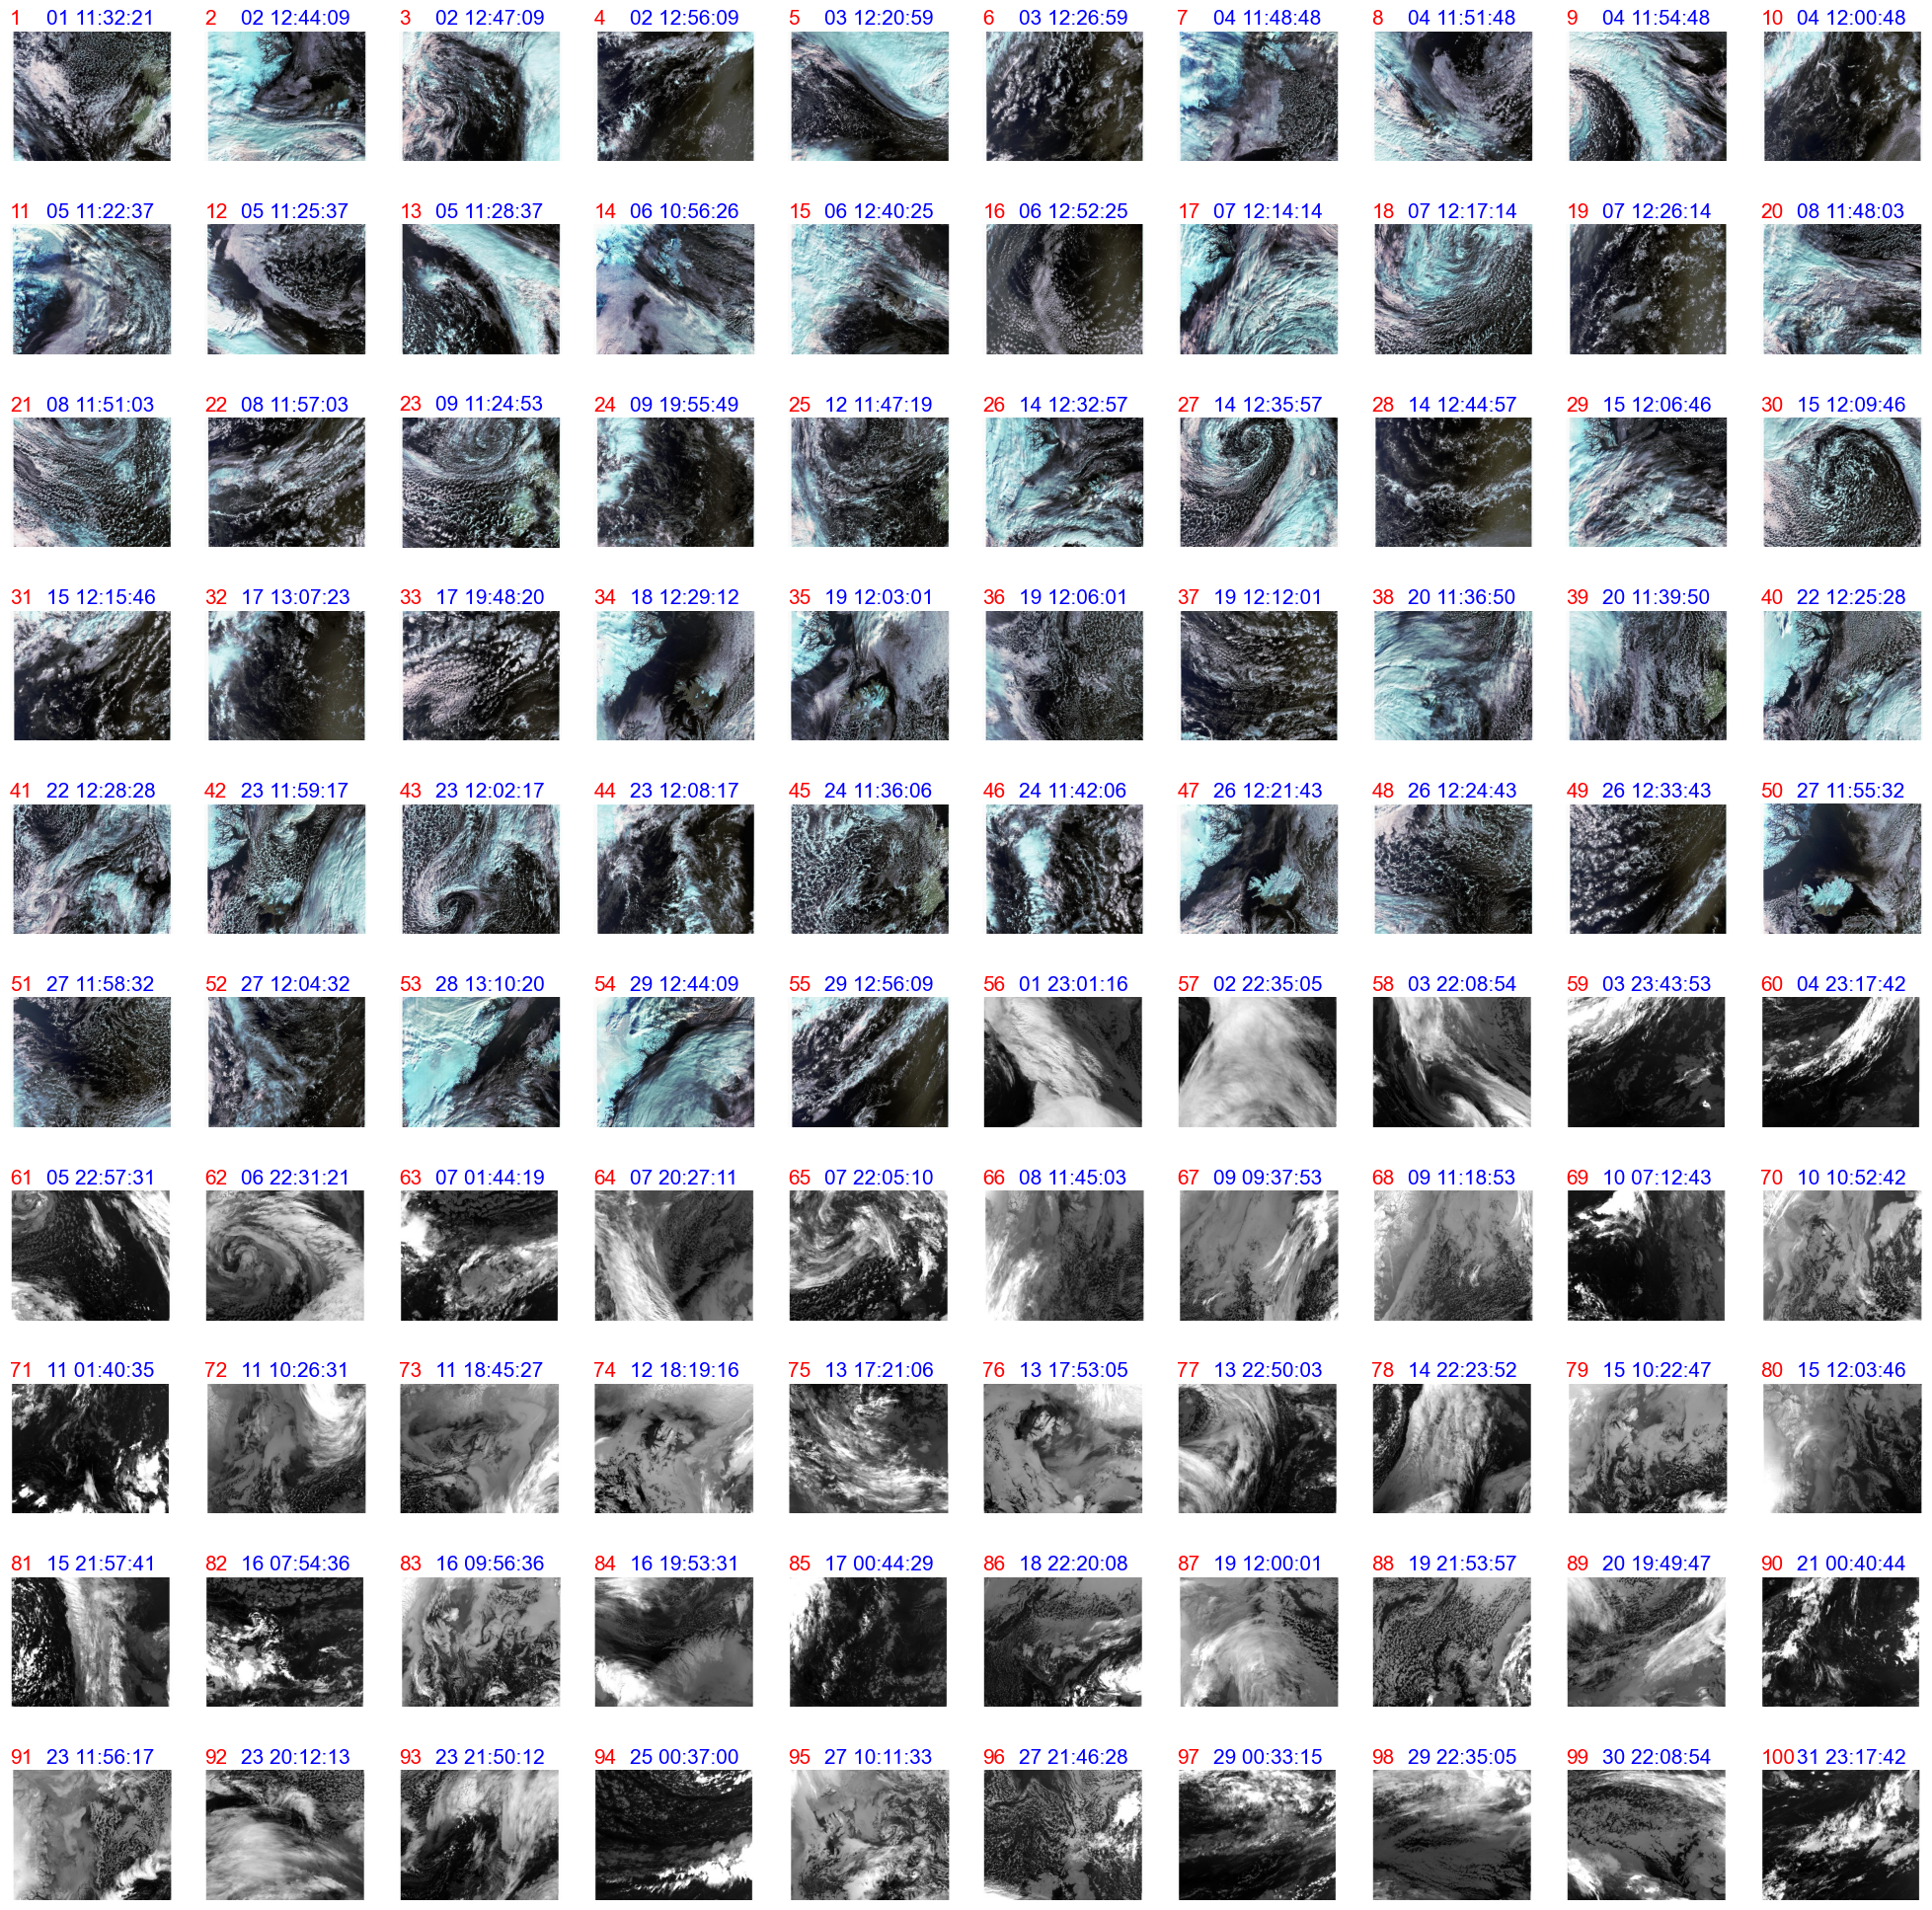
\includegraphics[width=0.8\paperwidth]{images/raw-output.png}
\caption{The raw satellite images at the locations where inference is chosen.}
\label{fig:frames-raw}
\end{figure*}

\begin{figure*}[htb]
\centering\includegraphics[width=0.8\paperwidth]{images/masks-output.png}
\caption{The mask images at the locations where inference is chosen.}
\label{fig:frames-mask}
\end{figure*}



%%%%%%%%%%%%%%%%%%%%%%%%%%%%%%%%%%%%%%%%%%%%%%%%%%%%%
\section{Conclusion}
%%%%%%%%%%%%%%%%%%%%%%%%%%%%%%%%%%%%%%%%%%%%%%%%%%%%%


In this paper, we provided a list of related activities for the MLCommons cloudmesh benchmark. It contains a list of activities that use the MLCommmons cloudmesh benchmark. It also includes a list of related research in regards to cloudmask detection in general. Through this document we hope that others have an easier time to get started and we can communicate activities related to the benchmark.

\begin{acks}

Work was in part funded by (a) NIST 60NANB21D151T  (b) NSF CyberTraining: CIC: CyberTraining for Students and Technologies from Generation Z with the award numbers 1829704 and 2200409 and NIST 60NANB21D151T , and (c) Department of Energy under the grant Award No. DE-SC0023452. The work from the UVA team was conducted at the Biocomplexity Institute and Initiative at the University of Virginia.

\end{acks}

%%
%% The next two lines define the bibliography style to be used, and
%% the bibliography file.

\bibliographystyle{ACM-Reference-Format}
\bibliography{vonLaszewski-cloudmask-related}

%%
%% If your work has an appendix, this is the place to put it.


\section*{Contributions}

The Ruochen Gu has conducted the work of identifying related research as a team member under AI for Scientific Research, a VIP group at NYU. He continued this work on voluntary basis due to his interest in this project. {\em GvL} has contributed significantly to porting cloudmask onto different machines while making the code portable and contributed the cloudmesh-ee workflow code, the cloudmesh StopWatch and integrated the cloudmesh timers and logging, into the code. He ran all benchmarks on Rivanna and the Desktop.   In discussions with Rutherford Lab a new accuracy value was introduced that was not included in the original version distributed by MLCommons. He also facilitated many hackathons with the NYU team. The work described here is cited in the NYU report.

\appendix

\onecolumn
\input{mask-table}


\end{document}
\endinput
%%
%% End of file `sample-sigplan.tex'.

